% Template for ICASSP-2021 paper; to be used with:
%          spconf.sty  - ICASSP/ICIP LaTeX style file, and
%          IEEEbib.bst - IEEE bibliography style file.
% --------------------------------------------------------------------------
\documentclass{article}
\usepackage{spconf,amsmath,graphicx}
\usepackage{subcaption}
\usepackage{amsthm}
\usepackage{amsfonts}
\usepackage{enumitem}
\usepackage{amssymb}
\usepackage{xcolor}
%\usepackage{esvect}
\usepackage{url}
\usepackage{graphicx}
\usepackage{subcaption}
\usepackage[ruled,vlined]{algorithm2e}
\usepackage{xcolor}
\usepackage[normalem]{ulem}
\usepackage{amsfonts}
\usepackage{amsmath}
\usepackage{amssymb}
\usepackage{xcolor}
\usepackage{amsthm}
%\usepackage{algorithm}
%\usepackage{algorithmicx}

\newtheorem{definition}{Definition}
\newtheorem{proposition}{Proposition}
\newtheorem{assumption}{Assumption}[section]
\newtheorem{corollary}[assumption]{Corollary}%[section]
\newtheorem{theorem}[assumption]{Theorem}%[section]
\newtheorem{lemma}[assumption]{Lemma}


\DeclareMathOperator{\Unif}{Unif}

\usepackage{hyperref}
\newcommand{\asaf}[1]{{\color{blue}{#1}}}
\newcommand{\asafc}[1]{{\color{blue}{[Asaf: #1]}}}

\newcommand{\A}[0]{\mathcal{A}}
\newcommand{\Var}[0]{\operatorname{Var}}
\newcommand{\SNR}[0]{\text{SNR}}
\newcommand{\E}[0]{\mathbb{E}}

\newcommand{\Cov}[0]{\operatorname{Cov}}
\newcommand{\R}[0]{\mathbb{R}}
% Title.
% ------
\title{Multi-target detection with the generalized method of moments}
%
% Single address.
% ---------------
\name{Ye'Ela Shalit$^\dagger$*, Ran Weber$^\dagger$*, Asaf Abas$^\ddagger$*, Shay Kreymer$^\dagger$*, and Tamir Bendory$^\dagger$
\thanks{* These four authors have contributed equally to this work.  \newline
S.K. is supported by the Yitzhak and Chaya Weinstein Research Institute for Signal Processing. T.B. is supported in part by NSF-BSF grant no. 2019752, and the Zimin Institute for Engineering Solutions Advancing Better Lives.}}
\address{$^\dagger$School of Electrical Engineering, Tel Aviv University, Tel Aviv, Israel\\
$^\ddagger$Department of Applied Mathematics, Tel Aviv University, Tel Aviv, Israel}
%
% For example:
% ------------
%\address{School\\
%	Department\\
%	Address}
%
% Two addresses (uncomment and modify for two-address case).
% ----------------------------------------------------------
%\twoauthors
%  {Ye'Ela Shalit*, Ran Weber*, Shay Kreymer* and Tamir Bendory\thanks{* These four authors have contributed equally to this work.  \newline
%S.K. is supported by the Yitzhak and Chaya Weinstein Research Institute for Signal Processing. T.B. is supported in part by NSF-BSF grant no. 2019752, and the Zimin Institute for Engineering Solutions Advancing Better Lives.}}
%	{School of Electrical Engineering \\
%	Tel Aviv University, Israel}
%  {Asaf Abas*}
%	{School of Mathematical Sciences\\
%	Department of Applied Mathematics\\
%	Tel Aviv University, Israel}

\begin{document}
%\ninept
%
\maketitle
%
\begin{abstract}
We consider the one-dimensional multi-target detection (MTD) problem of recovering a target signal from a noisy measurement that contains multiple copies of the signal, each randomly translated. Motivated by the structure reconstruction problem in single-particle cryo-electron microscopy, we focus on the high noise regime, where the noise hampers accurate detection of the signal occurrences. We develop a generalized method of moments framework to estimate the image directly from a measurement, and compare the framework to the method of moments through numerical experiments. We demonstrate signal recovery in highly noisy environments, and prove numerically the optimality of the generalized method of moments.
\end{abstract}
%
\begin{keywords}
Autocorrelation analysis, generalized method of moments, multi-target detection, cryo-electron microscopy.
\end{keywords}
%
\section{Introduction}
\label{sec:intro}
We study the multi-target detection (MTD) problem of estimating a target signal~$x \in \mathbb{R}^L$ from a noisy measurement that contains multiple copies of the signal, each randomly translated~\cite{bendory2019multi}, \cite{lan2020multi}, \cite{marshall2020image}, \cite{bendory2021multi}, \cite{kreymer2021two}, \cite{bendory2018toward}. Specifically, let~$y \in \mathbb{R}^N$ be a measurement of the form
\begin{equation}
\label{eq:model}
y[\ell] = \sum_{i=1}^{p} x[\ell - \ell_i] + \varepsilon[\ell],
\end{equation}
where \mbox{$\{\ell_i\}_{i=1}^{p} \in \{L + 1, \ldots, N-L\}$} are arbitrary translations, and~$\varepsilon[\ell]\overset{i.i.d.}{\sim} \mathcal{N}(0,\sigma^2)$. The translations and the number of occurrences of~$x$ in~$y$ are unknown. Figure~\ref{fig:measurements} presents examples of a measurement~$y$ at different signal-to-noise ratios (SNRs). We define~\mbox{$\text{SNR} := \frac{\|x\|_2^2}{L \sigma^2}$}.

\begin{figure}[!tb]
%	\begin{subfigure}[ht]{0.30\columnwidth}
%		\centering
%		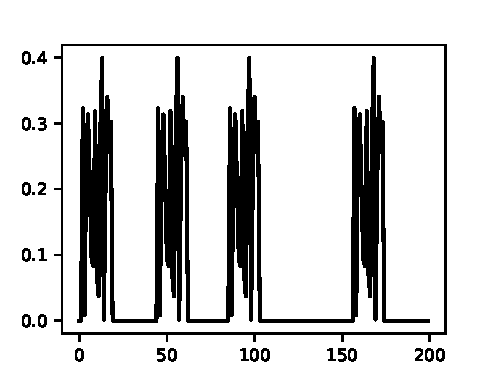
\includegraphics[width=\columnwidth]{figures/y_clean.pdf}
%		\caption{No noise.}
%	\end{subfigure}
%	\hfill
	\begin{subfigure}[ht]{0.49\columnwidth}
		\centering
		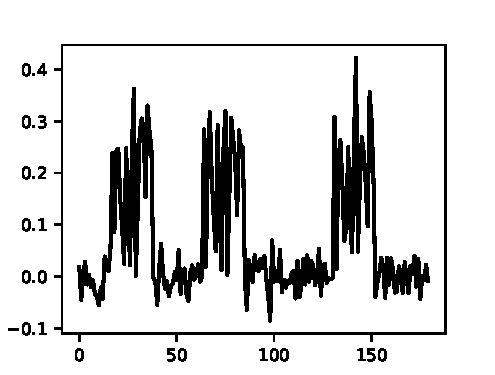
\includegraphics[width=\columnwidth]{figures/y_SNR50.pdf}
		\caption{$\text{SNR} = 50$.}
	\end{subfigure}
	\hfill
	\begin{subfigure}[ht]{0.49\columnwidth}
		\centering
		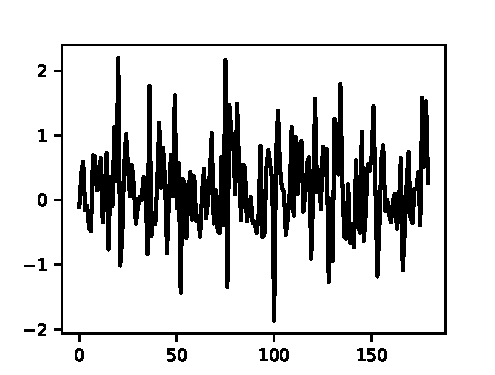
\includegraphics[width=\columnwidth]{figures/y_SNR01.pdf}
		\caption{$\text{SNR} = 0.1$.}
	\end{subfigure}
	\caption{Two measurements at different noise levels:~\mbox{$\text{SNR} = 50$} (left);~\mbox{$\text{SNR} = 0.1$} (right). Each measurement contains multiple copies of the target signal. In this work, our goal is to estimate the target signal directly from~$y$. We focus on the low SNR regime~(e.g., panel~(b)) in which the signal occurrences are swamped by the noise, and the locations of the signal occurrences cannot be detected reliably.}
\label{fig:measurements}
\end{figure}

The MTD model serves as a mathematical abstraction of the cryo-electron microscopy~(\mbox{cryo-EM}) technology for macromolecular structure determination~\cite{henderson1995potential},~\cite{nogales2016development},~\cite{bai2015cryo}. In a \mbox{cryo-EM} experiment \cite{frank2006three}, biological macromolecules suspended in a liquid solution are rapidly frozen into a thin ice layer. An electron beam then passes through the sample, and a two-dimensional tomographic projection is recorded. Importantly, the \mbox{2-D} location and \mbox{3-D} orientation of particles within the ice are random and unknown. This measurement, called \textit{micrograph}, is further affected by high noise levels and the optical configuration of the microscope.

In the current analysis workflow of \mbox{cryo-EM} data \cite{bendory2020single}, \cite{scheres2012relion}, \cite{punjani2017cryosparc}, the~\mbox{2-D} projections are first detected and extracted from the micrograph, and later rotationally and translationally aligned to reconstruct the~\mbox{3-D} molecular structure. This approach fails for small molecules, which induce low contrast, and thus low SNR. This makes them difficult to detect and align~\cite{bendory2018toward}, \cite{henderson1995potential}, \cite{bendory2020single}, \cite{aguerrebere2016fundamental}, rendering current \mbox{cryo-EM} algorithmic pipeline ineffective. For example, in the limit~\mbox{$\text{SNR} \rightarrow 0$}, reliable detection of signals' locations within the measurement is impossible~\cite[Proposition~3.1]{bendory2018toward}.

The MTD model was devised in \cite{bendory2018toward} in order to study the recovery of small molecules directly from the micrograph, below the current detection limit of \mbox{cryo-EM}~\cite{henderson1995potential},~\cite{d2021current}. An autocorrelation analysis technique (see Section~\ref{subsec:ac}) was implemented to recover \mbox{low-resolution}~\mbox{3-D} structures from noiseless simulated data under a simplified model. Autocorrelation analysis consists of finding a signal that best explains the empirical autocorrelations of the measurement,  by minimizing a {least-squares} (LS) objective. For any noise level, those autocorrelations can be estimated to any desired accuracy for sufficiently large~$N$. Computing the autocorrelations is straightforward and requires only one pass over the data, which is advantageous for massively large datasets, such as \mbox{cryo-EM} datasets~\cite{bendory2020single}.

Autocorrelation analysis is a variation of the method of moment (MoM), which is a classical statistical inference technique, tracing back to 1894~\cite{pearson1894contributions}. This work studies the \textit{generalized method of moments} (GMM) and specifically its application to the MTD problem. The GMM theory, which was first introduced in~\cite{Hansen1982}, shows that the GMM provides an optimal estimator, in comparison with other weighted LS objective function. As shown in previous works~\cite{abas2021generalized}, \cite{fan2018optimal}, \cite{roodman2009xtabond2}, the GMM estimator suggests a significant improvement in the estimation error.

The main contribution of this paper is in extending the MoM framework introduced in~\cite{bendory2019multi} by developing a GMM framework for the one-dimensional MTD problem. We devise an algorithm for the recovery of the target signal from a measurement, and demonstrate a successful reconstruction in noisy regimes~(see Section~\ref{sec:numerical}). Moreover, we corroborate the theory and present superior results for the GMM estimator in comparison with the MoM estimator for the MTD model. It is thus a significant step towards efficiently estimating a molecular structure directly from a noisy \mbox{cryo-EM} micrograph~\cite{bendory2018toward}.

\section{Mathematical framework}
\label{sec:math}
\subsection{Autocorrelation analysis}
\label{subsec:ac}
The autocorrelation of order~$q$ of a signal~\mbox{$z \in \mathbb{R}^{N}$} is defined as
\begin{equation}
A_z^q[\ell_1, \ldots, \ell_{q-1}] := \mathbb{E}_z\Big[\frac{1}{N} \sum_{i \in \mathbb{Z}} z[i] z[i + \ell_1] \cdots z[i + \ell_{q-1}]\Big],
\end{equation}
where~$\ell_1, \ldots, \ell_{q-1}$ are integer shifts. Indexing out of bounds is zero-padded, that is,~\mbox{$z[i] = 0$} out of the range~\mbox{$\{0, \ldots, {N-1}\}$}. In this work, we use the first three autocorrelations.

As~$N$ grows indefinitely, the empirical autocorrelations of~$z$ almost surely (a.s.) converge to the population autocorrelations of~$z$:
\begin{equation}
\lim_{N \rightarrow \infty} \frac{1}{N} \sum_{i \in \mathbb{Z}^2} z[i] z[i + \ell_1] \cdots z[i + \ell_{q-1}] \stackrel{\text{a.s.}}{=}A_z^q[\ell_1, \ldots, \ell_{q-1}],
\end{equation}
by the law of large numbers.

Our goal is to relate the autocorrelations of the measurement with the target signal~$x$. In particular, the first-order autocorrelation is defined as
\begin{equation}
\label{eq:AM1}
A_{y}^1 := \frac{1}{N} \sum_{i \in \mathbb{Z}} y[i].
\end{equation}
This is the mean of the measurement. The second-order autocorrelation of~$y$, \mbox{$A_{y}^2: \mathbb{Z} \rightarrow \mathbb{R}$}, is defined by
\begin{equation}
\label{eq:AM2}
A_{y}^2 [\ell_1] := \frac{1}{N} \sum_{i \in \mathbb{Z}} y[i] y[i + \ell_1],
\end{equation}
and the third-order autocorrelation~\mbox{$A_{y}^3: \mathbb{Z} \times \mathbb{Z} \rightarrow \mathbb{R}$} by
\begin{equation}
\label{eq:AM3}
A_{y}^3 [\ell_1, \ell_2] := \frac{1}{N} \sum_{i \in \mathbb{Z}} y[i] y[i + \ell_1] y[i + \ell_2].
\end{equation}


\subsection{Autocorrelations under the well-separated model}
\label{subsec:relations}
We discuss the \mbox{well-separated} case of the MTD problem, which was studied in~\cite{bendory2019multi}. In this case, we assume that each signal in the measurement~$y$ is separated by at least a full signal length from its neighbors. Specifically, we assume that
\begin{equation}
\label{eq:sep}
|\ell_{i_1} - \ell_{i_2}| \ge 2L - 1, \quad \text{ for all } i_1 \ne i_2.
\end{equation}

%Figure~\ref{fig:Micrograph_shifts}(a) presents an example of a measurement obeying the separation condition~(\ref{eq:sep}).
To compute the third-order autocorrelation~(\ref{eq:AM3}), we compute the product of~$y$ with its two shifts. Importantly, for~\mbox{$\ell$-s} in the range~$\mathcal{L} = \{0, \ldots, {L - 1}\}$, any given occurrence of~$x$ in~$y$ is only ever correlated with itself, and never with another occurrence.

In~\cite{bendory2019multi}, it was shown that under the separation condition~(\ref{eq:sep}), for any fixed level of noise~$\sigma^2$, density~$\gamma$ and signal length~$L$, in the limit~\mbox{$N \rightarrow \infty$} we have that
\begin{align}
\label{eq:well_separated_1st}
A_{y}^1 &\stackrel{\text{a.s.}}{=} \gamma A_{x}^1, \\
\label{eq:well_separated_2nd}
A_{y}^2 [\ell_1] &\stackrel{\text{a.s.}}{=} \gamma A_{x}^2 [\ell_1] + \sigma^2\delta[\ell_1], \\
\label{eq:well_separated_3rd}
A_{y}^3 [\ell_1, \ell_2] &\stackrel{\text{a.s.}}{=} \gamma A_{x} [\ell_1, \ell_2] \nonumber \\&+ \gamma A_{x}^1 \sigma^2 (\delta[\ell_1] + \delta[\ell_2] + \delta[\ell_1 - \ell_2]),
\end{align}
for~$\ell_1, \ell_2 \in \mathcal{L}$, where
\begin{equation*}
%\label{eq:delta}
\delta[\ell] = \begin{cases} 1 \text{ if } \ell = \vec{0}, \\ 0 \text{ otherwise}, \end{cases}
\end{equation*}
is the Kronecker delta function. Here,~$\gamma$ is the density of the target images in the measurement and is defined by
\begin{equation}
\gamma = p \frac{L}{N}.
\end{equation}



As such,~\mbox{(\ref{eq:well_separated_1st}) -~(\ref{eq:well_separated_3rd})} relate the autocorrelations of the measurement with those of the target signal~$x$. Importantly, the aforementioned relations between the autocorrelations of~$y$ and~$x$ do not directly depend on the location of individual signal occurrences in the measurement, but only through the density parameter~$\gamma$. Therefore, detecting the signal occurrences is not a prerequisite for signal recovery, and thus signal recovery is possible even in very low SNR regimes.

Next, we introduce the following notations
\begin{align}
\A_y^1 &:= A_y^1, \quad \A_x^1 := \gamma A_x^1, \nonumber\quad
	 \A_y^2 := \Big\{A_y^2[\ell]\Big\}_{\ell=0}^{L-1},\nonumber \\ 	\A_x^2 &:= \Big\{\gamma A_x^2[\ell]+ \sigma^2 \delta[\ell]\Big\}_{\ell=0}^{L-1},\nonumber\quad
	\A_y^3 := \Big\{A_y^3[\ell_1, \ell_2]\Big\}_{\ell_1,\ell_2=0}^{L-1},\nonumber \\
	\A_x^3 &:= \Big\{\gamma A_x^3[\ell_1, \ell_2] \nonumber\\&+ \gamma A_{x}^1 \sigma^2 (\delta[\ell_1] + \delta[\ell_2] + \delta[\ell_1 - \ell_2])\Big\}_{\ell_1,\ell_2=0}^{L-1}. \nonumber
\end{align}

\subsection{Signal recovery from autocorrelations}
Following~\cite{bendory2019multi}, \cite{lan2020multi}, \cite{marshall2020image}, \cite{bendory2021multi}, \cite{kreymer2021two} and based on the notations presented above, we formulate a non-convex least squares problem for estimating the signal~$x$ from the autocorrelations of the measurement~$y$:
\begin{align}
\label{eq:optimization}
\min_{x, \gamma > 0} &w_1 (\A_y^1 - \A_x^1)^2 \nonumber\\ +& w_2 \|\A_y^2 - \A_x^2\|_2^2 + w_3 \|\A_y^3 - \A_x^3\|_2^2,
\end{align}
where the weights were chosen such that each term is equally weighted, as suggested by~\cite{bendory2019multi}. This LS estimator serves as a benchmark to the GMM estimator, which is developed in the following section.

\subsection{Generalized method of moments}
\label{gmm}
\subsubsection{The GMM framework}\label{gmm:framwork}
In its most simplified form, the GMM generalizes~(\ref{eq:optimization}) by replacing the LS objective with specific optimal weights. This choice guarantees favorable asymptotic statistical properties, such as {the} minimal asymptotic variance of the estimation error.

Let us define the \textit{moment function},~\mbox{$f(\theta, y)\colon \Theta \times \R^r \to \R^q$}. The moment function is chosen such that its expectation value is zero only at a single point~$\theta=\theta_0$. Namely,
\begin{equation}\label{Eq-GMM-1}
	\E\left[f(\theta,y)\right] = 0 \quad \text{if and only if} \quad \theta = \theta_0.
\end{equation}
The moment function must satisfy this uniqueness condition~\eqref{Eq-GMM-1} and a few additional regularity conditions (which can be found in~\cite{Hansen1982}, \cite{abas2021generalized}). This flexibility enables the GMM to be applied to a wide range of problems, such as subspace estimation~\cite{fan2018optimal}.

In order to define the moment function for the MTD problem, we first define the $i$-th observation from the signal~$y$ as follows:
\begin{equation}
	y_i := [y[i],\ldots, y[i+L]].
\end{equation}
The choice of the moment function~$f(\cdot)$ must fulfill~(\ref{Eq-GMM-1}) using the defined samples~$y_i$. The natural choice of ~$f(\cdot)$ is
\begin{equation} \label{Eq-GMM-2}
	f(\theta,y_i) :=
	\begin{bmatrix}
		&\A_x^1 - \A_{y_i}^1\\
		&\A_x^2 - \A_{y_i}^2 \\
		&\A_x^3 - \A_{y_i}^3
	\end{bmatrix},
\end{equation}
where $\theta := [x, \gamma]$.
The estimated sample moment function is the average of~$f$ over~$N$ observations:
\begin{equation}\label{Eq-2-5}
	g_N(\theta) = \frac{1}{N} \sum_{i=1}^N f(\theta, y_i) = \begin{bmatrix}
		&\A_x^1 - \A_{y}^1\\
		&\A_x^2 - \A_{y}^2 \\
		&\A_x^3 - \A_{y}^3
	\end{bmatrix}.
\end{equation}
The GMM estimator is defined as the minimizer of the weighted LS expression
\begin{equation} \label{Eq-2-1}
	\hat{\theta}_N = \arg\min_{\theta \in \Theta} \ g_N(\theta)^T W_N g_N(\theta).
\end{equation}
Here, $W_N$ is a fixed positive semi-definite (PSD) matrix. Note that the LS estimator~(\ref{eq:optimization}) is a special case of~(\ref{Eq-2-1}).

\subsubsection{Large Sample Properties}\label{gmm:large}
Before presenting the statistical properties of the GMM, we fix notation. We denote by $\overset{p}{\to}$ and $\overset{d}{\to}$ convergence in  probability and in distribution, respectively. Let
\begin{equation} \label{eqn:cov_mat_S}
	S := \lim_{N\to \infty}\Cov\left[\sqrt{N}g_N(\theta_0)\right],
\end{equation}
be the covariance matrix of the estimated sample moment function~(\ref{Eq-2-5}) at the ground truth~$\theta_0$. We denote by $\{W_N\}_{N=1}^\infty$ a sequence of PSD matrices which converges almost surely to a positive definite (PD) matrix~$W$. Finally, the expectation of the Jacobian of the moment function at the ground truth~$\theta_0$ is denoted by $G_0 = \E\left[\partial f(\theta_0, y) / \partial \theta^T\right]$.

%Following~\cite{Hansen1982}, the large sample properties of the GMM estimator under the uniqueness of the parameter set~\eqref{Eq-2-4} are \tamir{as follows.}

The large sample properties of the GMM estimator were derived in~\cite{Hansen1982}, and are presented in the following theorem. The regularity conditions for this theorem can be found in~\cite{Hansen1982}, \cite{Hall2005}, \cite{abas2021generalized}.

\begin{theorem}\label{Thm-2-6}
	Under {the} regularity conditions, the GMM estimator satisfies:
	\begin{enumerate}[label={\Alph*}.]
		\item  \label{Thm-2-2}
		\textnormal{(Consistency)} $\hat{\theta}_N \overset{p}{\to} \theta_0$.

		\item \label{Thm-2-3} \textnormal{(Asymptotic normality)}
		\[\sqrt{N} ( \hat{\theta}_N - \theta_0) \overset{d}{\to} \mathcal{N}(0, M S M^T ),\] where $M =[G_0^T W  G_0]^{-1} G_0^T  W$.

		\item \label{Thm-2-5} \textnormal{(Optimal choice of a weighting matrix)} The minimum asymptotic variance of $\hat{\theta}_N$ is given by $(G_0^T S^{-1} G_0)^{-1}$ and is attained by $W = S^{-1}$.
	\end{enumerate}
\end{theorem}
Theorem~\ref{Thm-2-6} provides a matrix~$W$ {that} guarantees a minimal asymptotic variance of the estimator’s error. The covariance matrix~$S$ {of~(\ref{eqn:cov_mat_S}), which plays a central role in Theorem~\ref{Thm-2-6},} is required to be a PD matrix. Therefore, the moment function must be chosen so that~$S$ is full-rank. As in~\cite{abas2021generalized},  we remove the repeating entries of~$f$ (that appear due to the inherent symmetries of the autocorrelations).

It is important to note that in practice, the ground truth~$\theta_0$ is unknown a priori, so we cannot use the optimal weighting matrix. However as suggested in~\cite{abas2021generalized}, for our choice of the moment function~(\ref{Eq-GMM-2}), it is enough to apply the covariance on the empirical part,
	\begin{equation}\label{Eq-2-7}
		\Cov[g(\theta)] = \Cov\left[\left[A_{y_i}^1;\A_{y_i}^2;\A_{y_i}^3\right]\right].
	\end{equation}

\section{Numerical experiments}
\label{sec:numerical}
In this section, we present numerical comparisons for the estimators which was described in Section~\ref{sec:math}, the MoM and GMM estimators. The optimization problem~(\ref{eq:optimization}) was minimized using the~\mbox{Broyden-Fletcher-Goldfarb-Shanno}~(BFGS) algorithm, while ignoring the positivity constraint on~$\gamma$ (namely, treating it as an unconstrained problem).  We measure the estimation error by
\begin{equation}
\text{relative error}(x) = \frac{\|x - x^*\|_2}{\|x^*\|_2},
\end{equation}
where~$x^*$ is the true signal, and~$x$ is the estimated signal. The code to reproduce all experiments is publicly available at~\url{https://github.com/krshay/MTD-GMM}.


\subsection{Recovery error as a function of the measurement length}
\label{subsec:exp_size}
Figure~\ref{fig:err_size_experiment} presents recovery error as a function of the measurement size. We consider measurements with~\mbox{$\text{SNR} = 50$} in different sizes. The measurements are generated according to~(\ref{eq:model}) with density~$\gamma = 0.2$. The target signals in the measurements are of length~\mbox{$L = 21$}. We try to estimate the signal from 5 random initial guesses, and calculate the estimation error for the estimate whose final objective function is minimal. Then, we  calculate the median over 20 trials. As expected from the law of large numbers, both estimators' errors  decay as~$N^{-1/2}$. In addition, Theorem~\ref{Thm-2-6} provides the optimality of the GMM estimator over the MoM estimator, and indeed the median error of the GMM estimator is smaller than the error of the MoM estimator for all sizes.

\begin{figure}[!tb]
	\begin{subfigure}[ht]{\columnwidth}
		\centering
		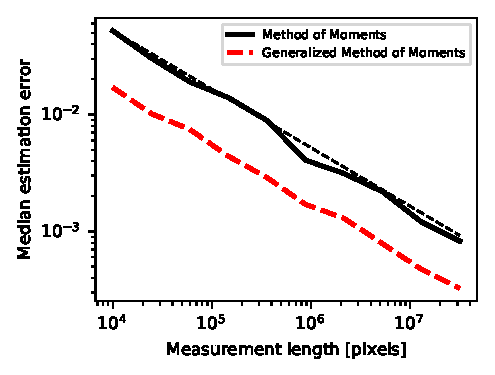
\includegraphics[width=\columnwidth]{figures/experiment_size_err.pdf}
	\end{subfigure}
	\caption{The median estimation error of recovering the signal~$x$, as a function of the measurement length~$N$, by: (a)~the MoM estimator; (b)~the GMM estimator.}
\label{fig:err_size_experiment}
\end{figure}

\subsection{Recovery error as a function of SNR}
Figure~\ref{fig:err_noise_experiment} presents recovery error as a function of SNR. We consider measurements of length~$1 \cdot 10^6$ with different SNRs. As in Section~\ref{subsec:exp_size}, the measurements are generated according to~(\ref{eq:model}) with density~$\gamma = 0.2$, the target signals in the measurements are of length~\mbox{$L = 21$}, and we try to estimate the signal from 5 random initial guesses and calculate the estimation error for the estimate whose final objective function is minimal. Then, we  calculate the \textbf{median} over \textbf{20} trials.
\begin{figure}[!tb]
	\begin{subfigure}[ht]{\columnwidth}
		\centering
		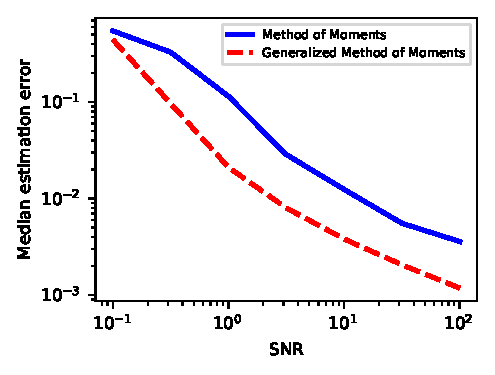
\includegraphics[width=\columnwidth]{figures/experiment_SNR_err.pdf}
	\end{subfigure}
	\caption{Median estimation error of recovering the signal~$x$, as a function of SNR, by: (a)~the MoM estimator; (b)~the GMM estimator.}
\label{fig:err_noise_experiment}
\end{figure}

\section{Conclusion}
\label{sec:conclusion}



\vfill
\newpage

\bibliographystyle{IEEEbib}
\bibliography{references}

\end{document}
